\renewcommand{\thechapter}{2}
\chapter{The EXO-200 Detector}

This chapter will describe the physical apparatus of the EXO-200 detector.  Section~\ref{sec:DetectorOverview} will give a broad overview of the detector.  Section~\ref{sec:DetectorBackgrounds} will identify the dominant backgrounds for $\beta\beta 0\nu$ decay, and sections~\ref{sec:DetectorPassiveBackgroundRejection} and \ref{sec:DetectorActiveBackgroundRejection} will describe methods used to mitigate these backgrounds.  The calibration system is described in section~\ref{sec:DetectorCalibration}.  We conclude with a description of the pulse and waveform readout subsystems in section~\ref{sec:DetectorReadout}, where discussion of the scintillation readout will be particularly important for subsequent chapters.  Throughout, the reader is referred to the detailed description in~\cite{detectorPartI} for more information.

\section{Overview of the EXO-200 Detector}\label{sec:DetectorOverview}

The EXO-200 detector is a cryogenic experiment containing $175$ kg of liquid xenon enriched to $80.6\%$ in $^{136}$Xe.  Of those $175$ kg of liquid xenon, $110$ kg are contained within the ``active'' volume where the detector is fully sensitive to deposited energy from $\beta\beta$ decay,~\cite{detectorPartI} and $94.7$ kg are contained within the fiducial volume where we believe the detector's response is well-understood.  Only fiducial xenon will be used in the search for $\beta\beta 0\nu$ decay; this means there are $3.39 \cdot 10^{26}$ atoms $^{136}$Xe which will be used for setting half-life limits.~\cite{NewEXObb0nPaper_2014}

\begin{figure}
\begin{center}
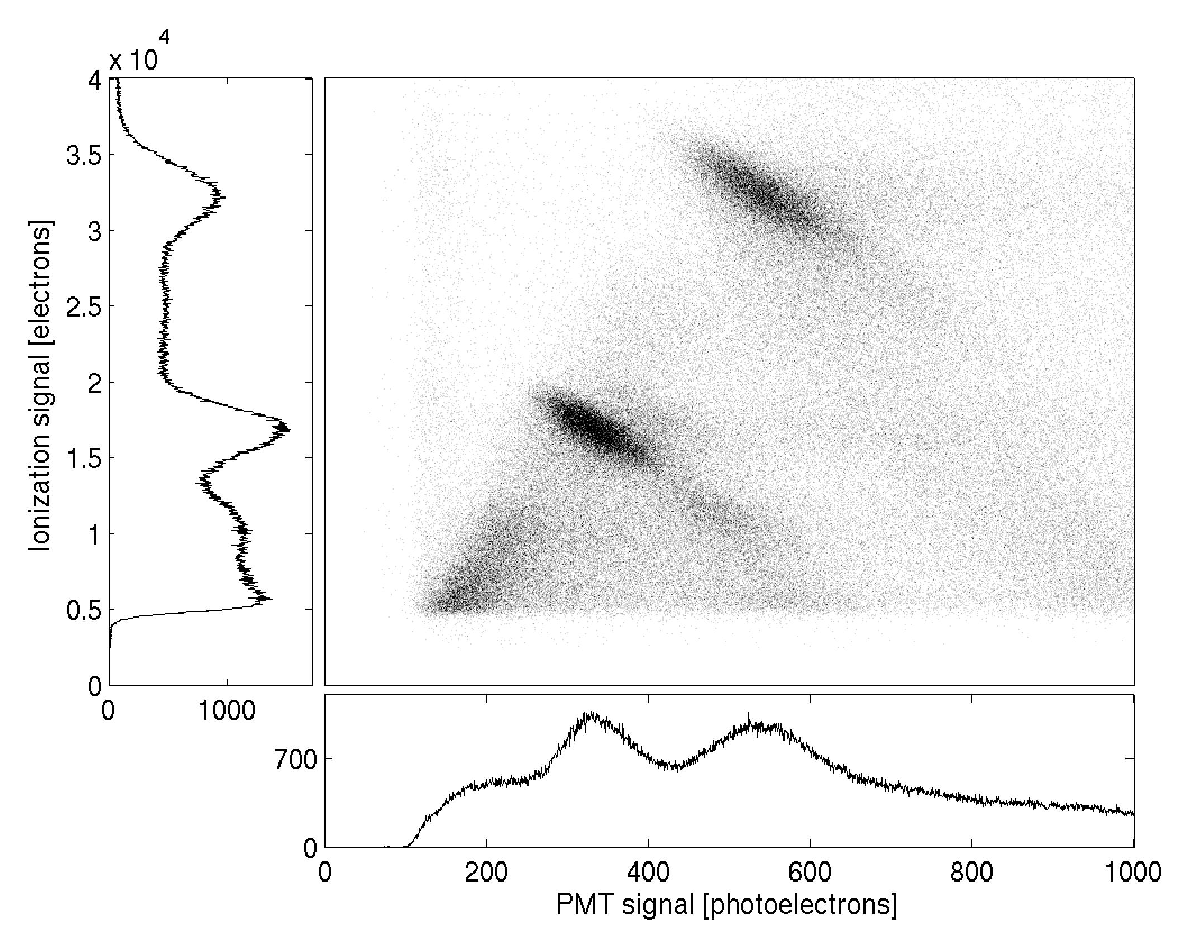
\includegraphics[keepaspectratio=true,width=\textwidth]{4kV_correl1.eps}
\end{center}
\renewcommand{\baselinestretch}{1}
\small\normalsize
\begin{quote}
\caption{A two-dimensional energy spectrum of scintillation and ionization from a testbed liquid xenon experiment under an electric field of $4$ kV/cm.  The spectrum is from a $^{207}$Bi source.  Figure reproduced from~\cite{PhysRevB.68.054201}.}
\label{fig:AnticorrelationInXenon}
\end{quote}
\end{figure}
\renewcommand{\baselinestretch}{2}
\small\normalsize

Energy deposits in xenon can be measured primarily in two ways: optical photons are emitted from the excitation and de-excitation of atomic electrons of xenon, and xenon atoms are ionized to produce free electrons.  It is well-known~\cite{PhysRevB.68.054201} that liquid noble element calorimeters show significant fluctuations in their separate production of scintillation photons and free electrons, but that these separate quantities are strongly anticorrelated.  As a result, is it possible to achieve far better energy resolution if both light and charge are independently measured than if only one is detected; figure~\ref{fig:AnticorrelationInXenon} illustrates this phenomenon in a testbed liquid xenon experiment, where it is apparent that using light and charge simultaneously lets us observe narrower gamma lines than either individually.

\begin{figure}
\begin{center}
\includegraphics[keepaspectratio=true,width=\textwidth]{TPCSchematic.eps}
\end{center}
\renewcommand{\baselinestretch}{1}
\small\normalsize
\begin{quote}
\caption{Schematic of the inner EXO-200 TPC.  Figure reproduced from~\cite{detectorPartI}.}
\label{fig:TPCSchematic}
\end{quote}
\end{figure}
\renewcommand{\baselinestretch}{2}
\small\normalsize

Scintillation will be produced from energy deposits in liquid xenon in all cases;~\cite{Thesis_EDahl} however, to observe free electrons we must exert an electric field on the xenon which drifts the electrons onto a collection anode.  The EXO-200 detector is shaped as a cylinder, and the required electric field is produced by placing a cathode grid in the center of that cylinder and anode wires along each of the two endcaps of the detector; such a detector is called a time projection chamber, or TPC.  The EXO TPC is shown in figure~\ref{fig:TPCSchematic}.  The light is collected by avalanche photo-diodes (see section~\ref{sec:DetectorReadout} for details) mounted on the endcaps behind the anode wires; the anode wires are thin, so the effect on light collection efficiency is minimal.

The cathode is maintained at a voltage of $8$ kV above the anode wire voltage.  Field shaping rings encircle the outside of the EXO cylinder to ensure that electric field lines are approximately parallel and the magnitude of the electric field is roughly constant in the bulk volume of xenon.  (Near the edges, non-uniformities in the electric field are believed to exist; these are a continuing topic of research.)  The cathode and anode wires are separated by roughly $20.4$ cm; after accounting for edge effects, we believe that the bulk volume of xenon has an electric field of roughly $374$ V/cm.

Electrons in liquid xenon drift at a velocity of $1.71$ mm/$\mu$s under an electric field of $375$ V/cm.  The maximum drift distance from the cathode to the anode is $198.4$ mm, resulting in a maximum electron drift time of roughly $116$ $\mu$s.  Free electrons are not absorbed by xenon -- as for other noble elements, xenon has a low electronegativity, so in a pure xenon detector electrons could drift unimpeded for the time necessary to reach the anode.  EXO-200 does have small quantities of electronegative impurities such as oxygen and methane; to minimize the concentration of these impurities, the xenon of EXO-200 is constantly circulated through a chemical purifier which extracts chemically active molecules and permits noble elements to pass through.~\cite{detectorPartI}

It is necessary to associate charge pulses with their corresponding scintillation pulses in spite of their time separation.  However, this is easily done provided the time between events is much longer than $116$ $\mu$s.  Thus, sources should be calibrated to produce a data rate in xenon no higher than roughly $1$ kHz.  By measuring the time difference between the observation of scintillation and the collection of charge, we can measure the position of the energy deposit along one dimension.  Our time resolution permits us to reconstruct this position coordinate with an accuracy of $0.42$ mm.~\cite{bb2nEXO2014}

\begin{figure}
\begin{center}
\includegraphics[keepaspectratio=true,width=\textwidth]{supportwithoutwires.png}
\end{center}
\renewcommand{\baselinestretch}{1}
\small\normalsize
\begin{quote}
\caption{Anode collection wires (u-wires) and induction wires (v-wires) from EXO-200.  (1) and (5) indicate the wire support frame; (2) indicates the wires themselves, constructed as gangs of three wires; (3) illustrates the attachment between wires and the support frame; (4) shows the return cables from the wires to the data acquisition system.  Figure reproduced from~\cite{detectorPartI}.}
\label{fig:UandVWiresCrossing}
\end{quote}
\end{figure}
\renewcommand{\baselinestretch}{2}
\small\normalsize

At the anode, there are two sets of parallel wire planes.  The first (closer to the cathode) parallel wire plane is called the ``v-wire'' plane, and the second plane is called the ``u-wire'' plane.  The voltages of the two wire planes are set so that no elecric field lines terminate on the v-wires, and all field lines instead penetrate through the v-wire plane and terminate on the u-wires.  When charge is deposited within the liquid xenon and drifts toward the anode, it induces a current on the v-wires as it passes by, and then produces a current on the u-wires as it is collected.

Figure~\ref{fig:UandVWiresCrossing} indicates the relative orientation of the u-wires and v-wires.  By detecting which (set of) wires observes a current pulse in both the u-wire and v-wire channels, it is possible to identify the two-dimensional location on the anode where the charge arrived.  Channels in each plane are $9$ mm wide; by taking advantage of signal sharing which sometimes occurs between u-wires and always occurs between v-wires, we are able to achieve position accuracy of $2.4$ mm perpendicular to the u-wires and $1.2$ mm perpendicular to the v-wires.~\cite{bb2nEXO2014}

Energy which appears to come from a single location is called a charge deposit ``cluster'' or ``site'', and events are classified according to the number of sites they produce (their ``multiplicity'') as either single-site or multi-site.  We will see in section~\ref{sec:DetectorActiveBackgroundRejection} that this is provides a powerful tool for background rejection.

This section has described how energy deposits in the liquid xenon are transformed into scintillation and charge, which are then observed by APDs and anode wires, respectively.  These observations are sufficient for us to reconstruct the positions and magnitudes of energy deposits in the liquid xenon.

\section{Backgrounds to \texorpdfstring{$\beta\beta 0\nu$}{Neutrinoless Double-Beta} Decay}\label{sec:DetectorBackgrounds}

$^{136}$Xe has a relatively high $Q$-value compared to most other $\beta\beta$ decays; in the neutrinoless mode the two emitted electrons will share $2456.7$ keV.  This means that the sensitivity of $T_{1/2}^{0\nu}$ to the mass of the neutrino is good in $^{136}$Xe, as was described in section~\ref{sec:NucPhysConstraintsFromBB0N}; it also means that energy spectrum around our $Q$-value will naturally be relatively free from most sources of background radiation.  This section will identify the types of background which can be expected to affect our $\beta\beta 0\nu$ search; subsequent sections will describe methods of mitigating those backgrounds.

It is common for alpha decays to have energies well in excess of our $Q$-value.  As a result, we might expect all alpha decays to be possible backgrounds to $\beta\beta 0\nu$.  However, alpha particles are stopped rapidly by even a small quantity of shielding, and as a result the only alpha decays which can be observed in the detector are those from sources which are dissolved into the xenon.  Radon is the only alpha-emitting noble element, and only $^{222}$Rn is sufficiently long-lived to diffuse into the xenon; as a result, we only expect $^{222}$Rn and its daughter products to contribute a significant quantity of alpha decays to the detector.

Cosmic rays produce high-energy muons; these are another source of high-energy backgrounds.  Muons will produce a streak of energy in the detector rather than discrete clusters; generally they will have sufficient energy to pass fully through the detector.  We can expect that such an event will look substantially different from a $\beta\beta 0\nu$ event, and generally will deposit substantially more energy than our $Q$-value as well.

More interesting are the associated by-products from the passage of such a high-energy particle, called spallation products.  Although high-energy muons can produce a range of fission products, the most significant spallation product of muons will be neutrons which can diffuse into the detector and activate materials there.  $^{134}$Xe and $^{136}$Xe are both present in significant quantities in the TPC, and by activation can be converted into the radioactive isotopes $^{135}$Xe and $^{137}$Xe respectively.  $^{135}$Xe has too little energy to be a background to $\beta\beta 0\nu$ decay, but $^{137}$Xe undergoes $\beta$ decay with a maximum energy of $4173$ keV.  We will see that indeed $^{137}$Xe is a significant source of background in our detector.

Some sources of background are intrinsic to the $\beta\beta 0\nu$ search.  Any isotope which can undergo $\beta\beta 0\nu$ decay can also undergo $\beta\beta 2\nu$ decay, and the endpoint of the $\beta\beta 2\nu$ spectrum is necessarily at our $Q$-value.  The only means of reducing background from $\beta\beta 2\nu$ is to improve the energy resolution of the detector so that fewer such decays can mimic $\beta\beta 0\nu$ decay.  Fortunately with the energy resolution exhibited by the EXO-200 detector, $\beta\beta 2\nu$ is subdominant to other backgrounds by many orders of magnitude.

Similarly, it is hypothetically possible for neutrino absorption to stimulate a $\beta\beta 2\nu$ decay by the reaction
\begin{equation}
2d + \nu_e \rightarrow 2u + 2e^- + \bar{\nu}_e
\end{equation}
which is obtained from the $\beta\beta 2\nu$ reaction by taking one neutrino from product to reactant in equation~\ref{eqn:bb2n_decay_reaction}.  The observable spectrum is similar to the standard $\beta\beta 2\nu$ spectrum, but with the endpoint shifted upward by the energy of the absorbed neutrino.  The cross-section for this reaction is excpected to be well below the cross-section for standard $\beta\beta 2\nu$, so this will be a negligible background well beyond the current generation of $\beta\beta$ detectors.

A gamma background which is particularly detrimental to EXO-200 comes from $^{214}$Bi, a member of the radium decay chain.  $^{214}$Bi emits a gamma particle at $2448$ keV, which with our energy resolution is indistinguishable from our $Q$-value.  It will occur as a daughter product of $^{226}$Ra, which has a half-life of $1600$ years and generally will be supported by $^{230}$Th ($75,000$ years), $^{234}$U ($250,000$ years), and ultimately by $^{238}$U ($4.5 \cdot 10^9$ years) which has a primordial abundance in the Earth's crust and most natural materials.

Most other backgrounds to $\beta\beta 0\nu$ will be gamma decays from $^{208}$Tl, a member of the thorium decay chain.  $^{208}$Tl emits a gamma particle at $2614.5$ keV; with our $Q$-value of $2456.7$ keV, the two energies are separated by $157.8$ keV.  The energy resolution (in $\sigma/\text{mean}$) of EXO-200 has typically been $1.5-2\%$ at these energies, meaning that separation between the central values of the gamma lines will be $3-4\sigma$.  The thorium decay chain is supported by $^{232}$Th, which has a half-life of $14$ billion years and has a significant abundance in most natural materials; we may expect it to contribute a significant fraction of our radioactive backgrounds, and as a result we may expect that some events from the $2615$ keV $^{208}$Tl line will leak across those $3-4\sigma$ and act as backgrounds.  Keeping our energy resolution at or below $1.5\%$ may be of significant interest in reducing contamination from this gamma line.

The compton edge is a well-known feature of gamma decay spectra; it originates from gammas which enter a calorimeter, scatter once, and escape from the detector.  The maximum energy which a gamma of incident energy $E_{inc}$ can deposit in a single compton scatter is:
\begin{equation}
E_{dep} = \frac{2E_{inc}^2}{m_e c^2 + 2E_{inc}}.
\end{equation}
When the incident gamma has an energy of $2615$ keV, the compton edge will lie at $2382$ keV, or only $74.5$ keV below our $Q$-value.  Using the same estimate that our energy resolution is around $1.5-2\sigma$ at these energies, this separation is only around $1.5-2\sigma$.  It is clear that improving our energy resolution may have a strong impact on background contamination by improving separation from the compton edge of the $^{208}$Tl as well as its full deposit line.

We have here identified some of the primary backgrounds which can be expected in the EXO-200 detector, noting particularly those which can be significantly reduced through improvements to the energy resolution.  The following sections will identify some of the mechanisms used to further minimize these backgrounds.

\section{Passive Background Rejection}\label{sec:DetectorPassiveBackgroundRejection}

When we describe the methods by which backgrounds to $\beta\beta 0\nu$ are reduced, we can distinguish between two classes: passive methods in which backgrounds are reduced by reducing the amount of background reaching the xenon in the first place, and active methods in which backgrounds are observed by the detector but discriminated from $\beta\beta$ signal based on identifying characteristics.  In this section, passive methods will be described; section~\ref{sec:DetectorActiveBackgroundRejection} will describe the active methods of background rejection.

\begin{figure}
\begin{center}
\includegraphics[keepaspectratio=true,width=\textwidth]{XrayAttenuationXenon.png}
\end{center}
\renewcommand{\baselinestretch}{1}
\small\normalsize
\begin{quote}
\caption{X-ray attenuation lengths in xenon.  Compton (incoherent) scattering, pair production, and photoelectric absorption are shown, along with their combined attenuation length; coherent (Rayleigh) scattering is omitted because it produces no observable energy deposit.  The vertical axis, in $\text{cm}^2/\text{g}$, can be multiplied by the density of the xenon to derive an attenuation factor per unit length.  Figure produced by~\cite{XcomXenonAttenuation}.}
\label{fig:XrayAttenuationXenon}
\end{quote}
\end{figure}
\renewcommand{\baselinestretch}{2}
\small\normalsize

The simplest and most immediate method of reducing the presence of backgrounds is by exploiting the self-shielding properties of xenon.  The xenon itself is extremely pure due to the easy of chemical purification; as a result most backgrounds will be external to the xenon.  Since external gammas are attenuated by dense materials such as liquid xenon, we can expect that the xenon near the center of the detector will be exposed to less background than the xenon near the TPC walls.  This is one of the primary advantages of xenon as a source: it is easy to construct a large monolithic detector, maximizing the quantity of xenon which is shielded from the walls.

Figure~\ref{fig:XrayAttenuationXenon} shows the attenuation lengths of gammas at a range of energies in xenon.  Photoabsorption and pair production both convert the gamma entirely into short-ranged electron and positron carriers; compton (incoherent) scattering results in only some deposited energy, with the rest remaining in the gamma which will rebound and continue on its path.  Liquid xenon has a density around $3$ g/cm$^3$, which means that the minimum attenuation factor is roughly $0.1/\text{cm}$ at energies around $4$ MeV.  Unfortunately, this is the same order of magnitude as our $Q$-value at $2456.7$ keV, which means that at the energy of interest to us self-shielding is minimally effective.  Nevertheless, there will still be some reduction in backgrounds deeper in the interior of the xenon, and lower-energy gammas will be attenuated more effectively.

To reduce the quantity of background around the detector, all materials near the xenon were carefully screened for radioactive contamination.  Backgrounds from $^{40}$K, $^{232}$Th, and $^{238}$U were cataloged for all materials which have unshielded line-of-site access to the detector system.  Requirements for $^{238}$U were particularly stringent because its daughter products include the $^{214}$Bi background which cannot be resolved from $\beta\beta 0\nu$ decay.  For the copper of the TPC vessel and the lead shielding around the detector apparatus, samples from a range of companies and mines were tested to locate an optimal choice of material source.  For the wires which were placed into the TPC, a range of manufacturing methods were tested; improvements to a photo-etching scheme were identified which led to a reduction in background from these materials.  This thorough material screening research is one of the distinctive processes which has enabled EXO-200 to fully reach its background targets.  Details of the selection and quantification of material radioactivity can be found in~\cite{MaterialsCatalog}.

Beyond selecting extremely clean materials, it is possible to reduce backgrounds by minimizing the mass of these external materials.  Most notably, EXO-200 is constructed with a copper TPC which in most places is only $1.37$ mm thick; to maintain structural integrity, supporting structures are welded to the TPC where needed, and it was possible to keep the total mass of copper below $30$ kg.~\cite{detectorPartI}

Some materials were dispensed with entirely.  Typically, silicon APDs are encapsulated with ceramic to isolate them from water contamination and provide electrical insulation.  However, this ceramic material would have contributed backgrounds.  Instead, the APDs were delivered ``bare,'' without any encapsulation, and protected from water by storing them in a dry-nitrogen container.  Liquid xenon itself serves as an excellent electrical insulator, ensuring the APDs would function properly during detector operations.~\cite{EXOLAAPD}

\begin{figure}
\begin{center}
\includegraphics[keepaspectratio=true,width=\textwidth]{triplet.jpg}
\end{center}
\renewcommand{\baselinestretch}{1}
\small\normalsize
\begin{quote}
\caption{Wire triplet, read as one channel.  Figure from~\cite{detectorPartI}.}
\label{fig:WireTriplet}
\end{quote}
\end{figure}
\renewcommand{\baselinestretch}{2}
\small\normalsize

\begin{figure}
\begin{center}
\includegraphics[keepaspectratio=true,width=\textwidth]{PlatterWGO7.png}
\end{center}
\renewcommand{\baselinestretch}{1}
\small\normalsize
\begin{quote}
\caption{APDs ganged together (bottom right).  Wiring to the front-end electronics are visible as yellow ``tape.''  Figure from~\cite{detectorPartI}.}
\label{fig:APDgang}
\end{quote}
\end{figure}
\renewcommand{\baselinestretch}{2}
\small\normalsize

Another example of material avoidance comes from the cabling from wires and APDs to the electrical amplifiers and digitizers.  These electronics contain many high-background plastics and other complex materials, so they were placed outside the lead shielding rather than placing them close to the TPC.  Wires connect the sensors in the TPC to these electronics; ordinarily such long wires would need to be shielded by coaxial cabling to minimize cross-talk noise.  However, the coaxial cabling was expected to contribute a high quantity of radioactive background, and was omitted; instead wires are partially shielded by surrounding them with inactive wires which reduce cross-talk noise.  Furthermore, the total number of wires needed was reduced by ganging together triplets of u- and v-wires and groups of six or seven APDs into single channels; this reduced the fineness of event information available in analysis, but reduced the quantity and complexity of material placed near the detector.  See the wire gangs in figure~\ref{fig:WireTriplet}; APD gangs and wiring to external electronics are visible in figure~\ref{fig:APDgang}.~\cite{detectorPartI}

We can imagine the TPC being shielded by nested layers of clean material designed to prevent backgrounds from reaching the xenon.  In the innermost layer, HFE-7000 refrigerant is used to maintain the detector at liquid xenon temperatures and maintain similar pressures inside and outside of the copper vessel walls.  However, the HFE has a significant quantity of hydrogen, which makes it an excellent stopping agent for thermal neutrons.  The refrigerant layer is more than $50$ cm thick, so most neutron products of muons have time to thermalize and absorb onto hydrogen before reaching the TPC and producing $^{137}$Xe.~\cite{detectorPartI}

The following layer of shielding is lead.  This is a common approach for low-background experiments due to the high density of lead, which enables it to stop gammas in a short distance.  Lead bricks surround the detector on all sides; the bricks were designed with an interlocking shape to ensure no seams between bricks left a line-of-sight path from external sources into the TPC.  In the front of the detector, where plumbing must enter and exit the detector through the first lead wall, a second lead wall is assembled with the purpose of blocking any line-of-sight paths into the TPC through the plumbing gaps of the first wall.~\cite{detectorPartI}

Outside of the lead shielding, restrictions on materials are less stringent; however, control over the presence of materials is still desired.  The entire apparatus is contained inside a class-1000 clean room facility.  Entire facility is located in the Waste Isolation Pilot Plant (WIPP) facility, a DOE-owned waste repository located in a salt mine in Carlsbad, NM.  The overburden of the facility is $1585$ m water-equivalent, leading to a significant reduction in muon rate compared to the rate observed on the Earth's surface.  \textcolor{red}{Would be nice to find a plot of muon intensity vs depth mwe.}

These passive approaches have all been demonstrated to reduce the rate of backgrounds depositing energy in the liquid xenon.  The following section will describe an active set of background-rejection approaches.

\section{Active Background Rejection}\label{sec:DetectorActiveBackgroundRejection}
	Charge/Light Ratio rejects alphas.
	SS/MS ratio rejects significant fraction of gammas.
	Resolution as background rejector.

\section{Calibration Systems}\label{sec:DetectorCalibration}
	Source calibrations
	Laser calibrations
	Charge injection runs
	External charge calibrations possible.

\section{Pulse Amplification and Waveform Readout}\label{sec:DetectorReadout}
	APDs [Include detail of APD operation; introduce notation consistent with denoising chapter]
	Wires
	No coax cables [noisy]
	DAQ [e-boards might be noisy -- can I reference something?]
	Trigger (2ms most of the time, not always)



\textcolor{red}{Scintillation as limiting factor on resolution [here or expanded treatment in denoising chapter]}








The properties of $^{136}$Xe make it an excellent material to use for the search for $\beta\beta 0\nu$ decay.  It has a relatively high $Q$-value of $2457.8$ keV; this leads to a favorable phase factor which increases the strength of a half-life limit in constraining $\left<m_{\beta\beta}\right>$, and also ensures that most radioactive backgrounds do not emit radiation energetic enough to mimic our signal.  It is a noble element, meaning it can be enriched in a centrifuge with minimal complications and expense, and it can also be purified chemically with ease.  Its natural abundance is $8.9\%$, which also reduces the cost of enrichment.

Unlike many $\beta\beta$ candidates, Xenon has an advantage that it responds to energy deposits by emitting scintillation and, if an electric field is applied, producing free electrons.  As a result, we do not need to dissolve or dope the Xenon with any other material -- pure Xenon can serve as both the source and detector of $\beta\beta$ decays.  As a result, it is feasible to construct EXO-200 as a large monolithic detector.

Because Xenon itself can be purified so effectively, we do not expect to see significant radioactive backgrounds dissolved in the Xenon itself -- most backgrounds will be external.  Furthermore, Xenon is quite dense; liquid Xenon weighs $3.0$ g/cm$^3$.  As a result, the Xenon can act as a self-shielding source for which most external backgrounds interact before reaching the interior of the Xenon.  However, here the energy scale of interest hurts us:  the attenuation length of gammas is quite long at our $Q$-value \textcolor{red}{Figure of gamma attenuation}, so many gamma backgrounds will still penetrate through our detector.

Another form of background rejection can come from the nature of the energy deposits.  At our $Q$-value, the dominant mode of interaction is by Compton scattering, meaning that we expect most gamma particles to deposit energy in more than one location.  By contrast, $\beta$ and $\beta\beta$ decay inside the Xenon will generally deposit all of their energy in one highly localized ``cluster''.

To take advantage of this difference in interactions, the detector is sensitive to fully three-dimensional positions in the following way:
\begin{itemize}
\item We have stated that both light and charge are detected; this is accomplished by exerting an electric field on the Xenon which drifts free charge onto one of a number of anodes.  The drift velocity of electrons at our field is $1.71$ mm/$\mu$s, and our digitization is at a rate of $1$ MHz, so the position of an energy deposit along the electric field lines can be determined from the separation between charge and light signals to an accuracy on the order of $2-3$ mm.
\item The anode consists of two planes of parallel wires, one at each endcap of the detector.  By detecting which wire collects the charge, we can determine the position of the deposited charge in a direction orthogonal to the wire axis and electric field.  Wires are spaced by a $3$mm pitch; however, wire signals are only digitized from groups of three wires, so the effective accuracy of reconstruction in this direction will be approximately $3-4$ mm.
\item A second set of parallel wire planes is placed in front of the charge collection wires, and is voltage-biased so that no electric field lines terminate on it and it does not collect any charge.  However, it will still be sensitive to the induced charge signal caused by ionization passing through these wire planes on its way to the collection wires.  The so-called ``induction'' wires also have a pitch of $3$mm and are also digitized in groups of three wires, so the effective accuracy of reconstruction in the third direction will also be approximately $3-4$mm.
\end{itemize}
We can see that by combining all data, we are able to locate the positions of energy deposits with a three-dimensional accuracy of roughly $3-4$mm.  Energy which appears to come from a single location is called a charge deposit ``cluster'' or ``site'', and events are classified according to the number of sites they produce (their ``multiplicity'') as either single-site or multi-site.  By classifying events in this way, we find that the majority of $\beta\beta$ events are single-site and the majority of gamma events are multi-site; this distinction thus enables us to further reduce our rate of background.




Xenon is a convenient material to study because it is a noble element, making it easy to purify chemically.  It has no long-lived radioactive isotopes, so there is no concern of cosmogenic activation of the Xenon while aboveground.  It has a fairly high Q-value of 2.458 MeV, giving it a larger phase-space for its decay products and putting its peak out of reach of many common backgrounds.  Xenon also provides two means to measure energy from a decay:  under the influence of an electric field, ionization charge in pure Xenon will drift; and regardless of electric field, excited Xenon scintillates.  The ratio of scintillation to ionization depends on electric field and the density of the energy deposit; thus, at high enough electric field discrimination is possible between high-energy-density $\alpha$-decay and lower-energy-density $\beta$- and $\gamma$-decay.  Another benefit of Xenon is that, since it can act as an energy detector in its pure gaseous or liquid state, it is easy to make a large monolithic Xenon detector.  We will here review how the EXO-200 experiment has been constructed to exploit these properties and explore down to interesting neutrino masses.



The core of the EXO-200 detector is a cylindrical time-projection chamber (TPC), depicted in Figure~\ref{fig:TPCSchematic}, under a potential of roughly 400 V/cm.  The electric field is shaped to be parallel to the axis of the TPC throughout its fiducial volume.  The cathode is located in the middle of the TPC, and charge is collected on grids of parallel wires on either end of the TPC, giving a high-quality probe of the total ionization charge and location along one axis.  Also on both ends of the TPC, in front of these collection wires is another grid of parallel wires, orthogonal to the collection wires, which identifies an induced signal from passing ionization charge to give another position coordinate.  Finally, on both endcaps of the TPC are many large-area avalanche photodiodes (LAAPDs) which can detect the scintillation light from the primary decay~\cite{EXOLAAPD}.  The time difference between scintillation and charge collection gives a third position coordinate from a decay, and the scintillation also can give a secondary measurement of the energy of the deposit.  As noted above, comparing the scintillation and collected ionization allows $\alpha$-decays to be identified, removing one broad source of backgrounds.

The Xenon must be kept extremely pure, both to reduce backgrounds and to permit the ionization charges to drift farther with less attenuation.  To accomplish this, the detector has two pipes feeding into it so that Xenon may be circulated out of the detector continuously for repurification.  This is done using SAES Zirconium getters, which filter out all chemically reactive elements and return only noble elements.  Radioactive isotopes which are not filtered out are $^{85}$Kr (which has a Q-value much lower than that of $^{136}$Xe, making it fairly harmless) and all forms of Radon (some of whose daughter products can deposit energy around the Q-value of $^{136}$Xe).

The TPC itself is made of oxygen-free high-thermal-conductivity (OFHC) copper that was kept under concrete shielding during its time aboveground to protect it from neutron-induced activation.  Nevertheless, the copper may be a significant source of backgrounds in the energy range of interest, primarily due to natural contamination by $^{40}$K, $^{238}$U and $^{232}$Th~\cite{MaterialsCatalog}.  To mitigate this, significant effort has been expended in making the copper walls as thin as possible, averaging $1.5$ mm thick.  The ductility of copper makes such thin walls technically challenging, and a significant infrastructure has been developed to maintain the pressure of ultrapure HFE coolant, in which the TPC is immersed, so that the pressure difference can be controlled to $\sim 10$ torr.

Other significant sources of background may be the charge collection wires that pass through the TPC and the LAAPDs on its ends.  Both backgrounds have been minimized by limiting the total mass and carefully selecting materials to use.  The charge collection wires are photo-etched from phosphor bronze; the etching process was found to contribute to surface contamination, which was minimized by the use of clean etching agents and the use of a more aggressive cleaning procedure after etching~\cite{MaterialsCatalog}.  The LAAPDs are designed to minimize the radioactive contamination they introduce.  They were designed without standard ceramic encapsulation; instead the LXe is itself relied upon to insulate them.  Additionally, Aluminum used in the LAAPDs was found to be high-background, and was replaced with an acceptable substitute.  These efforts have reduced the activity introduced by the LAAPDs~\cite{MaterialsCatalog}\cite{EXOLAAPD}.

